\documentclass[a4paper]{article}
\usepackage[utf8]{inputenc}
\usepackage{csquotes}
\usepackage[ngerman]{babel}
\usepackage{biblatex}
\usepackage{float}
\usepackage{graphicx}
\usepackage{epstopdf}
\usepackage{subfigure}
\usepackage{array}
\usepackage{booktabs}
\makeatletter
\renewcommand\@ptsize{13}
\makeatother
\usepackage{extsizes}
%\setcounter{secnumdepth}{-1} 
\usepackage{hyperref}
\usepackage{nameref}
\usepackage{minted}
\makeatletter
\renewcommand\paragraph{%
   \@startsection{paragraph}{4}{0mm}%
      {-\baselineskip}%
      {.5\baselineskip}%
      {\normalfont\normalsize\bfseries}}
\makeatother
\usemintedstyle{friendly}
\bibliography{bibliography}
\title{Semesterarbeit im Fach Programmieren fortgeschrittene Konzepte}
\author{Dominik Eckelmann, Matr.-Nr.: 785856}
\date{\today}

\begin{document}

\sloppy

\begin{figure}[H]
	\centering
	
\includegraphics[width=0.7\textwidth]{beuth.eps}
	\maketitle
\end{figure}

\newpage
\tableofcontents

\newpage
\section{Einleitung}
Wenn man sich Quelltexte von anderen Autoren ansieht oder eigene Quelltexte, die man vor langer Zeit geschrieben hat, wird man feststellen, dass sich der schreibstiel stark unterscheiden kann. Man merkt, dass einige Quelltexte leichter zu verstehen sind als andere auch wenn die Thematik ähnlich komplex ist. Mit dieser Lesbarkeit von Quelltexten haben sich schon viele erfahrene Programmierer beschäftigt\cite{Knuth, Heusser, Kamp, Martin, reed} aber keine von ihnen hat eine goldene Regel gefunden wie man einen leicht verständlichen Quelltext schreibt. Genauso wenig gibt es eine Metrik mit der sich die Lesbarkeit verlässlich bestimmen lässt.

In dieser Arbeit werden die Paper \enquote{Coding Guidelines: Finding the Art in the Science} von Robert Green und Henry Ledgard\cite{Green}, sowie das Paper \enquote{Reading, Writing, and Code} von Diomidis Spinellis\cite{Spinellis} betrachtet. Beide Paper behandeln das Schreiben von Quelltext. Dabei stehen keine komplexen technischen Herausforderungen im Vordergrund sondern allein der Quelltext. Was steht drin, wie kann man ihn schreiben.

Zudem wird eine Coding Convention erstellt werden, der als Leitfaden für Programmierer dienen soll, einen guten Quelltext zu schreiben. Aufgrund der gesammelten Erfahrung bei der Erstellung soll festgestellt werden, in wieweit eine Coding Convention zu einem besseren Quelltext führen kann.

Häufig wird in Arbeiten das erstellen von guten Quelltexten als eine \enquote{Art}, also Kunst, gesprochen. Auch diesem Umstand soll auf den Grund gegangen werden.



\section{Fachliche Grundlagen}

Dieses Kapitel beschäftigt sich vor allem mit Quelltext. Wer schreibt ihn, wie wird er erstellt, wie sieht er aus, welche Entwicklungen hat es dabei gegeben. Was gibt es für Ansätze um einen langen Quelltext einheitlich aussehen zu lassen und vor allem wodurch zeichnet sich guter Quelltext aus und was sind die Auswirkungen von schlechtem. Zu guter Letzt werfen wir noch einen Blick auf die Wörter \enquote{Art} und \enquote{Science}, die in diesem Zusammenhang oft verwendet werden.

\subsection{Quelltext und der Autor}

Quelltext ist eine für den Computer verständliche Form
eines Arbeitsablaufes. Er kann durch einen Compiler in Maschinencode übersetzt werden.
In den meisten Fällen ist er in Textform verfasst und für den Menschen lesbar.

In einem Softwareprojekt ist er die detaillierteste Spezifikation der zu erstellenden
Software und all ihrer Komponenten. Alles wird in ihm so eindeutig beschrieben,
dass ein Computer ihn umsetzen kann. Das aus der modellgetriebenen Entwicklung
bekannte UML hat das Ziel den Quelltext durch definierte Modelle zu ersetzen.
Diese sind aus heutiger Sicht aber noch nicht als Quelltext Ersatz geeignet,
da die UML nicht genau genug ist und in ihr bestimmte Implementierungsdetails verloren gehen.
 \cite[S. 26]{Martin}

Der Autor dieser genauesten Spezifikation, des Quelltextes, ist der Programmierer.

\subsection{Wandel in der Entwicklung von Quelltexten}


In den Anfängen des Computerzeitalters war der Programmierer meistens der einzige
Leser seiner Programme. Hauptaugenmerk lag auf der Funktion des Programmes
und dem effizienten Umgang mit den Ressourcen, die zu dieser Zeit noch sehr knapp waren.
 Damals gab es noch keine Objekt-Orientierten-Sprachen. Zudem waren die Arbeitsumgebungen der Entwickler
wesentlich bescheidener als in der heutigen Zeit. Quelltexte wurden im ASCII-Code
kodiert und es passten lediglich 80 Zeichen auf eine Bildschirmzeile.

Durch die rasante technische Weiterentwicklungen ist ein Programmierer heutzutage keiner
80 Zeichen Zeile mehr unterworfen. Auch muss nicht mehr auf jedes Bit Speicherverbrauch
optimiert werden. Die Werkzeuge zur Softwareentwicklung haben sich auch verbessert. So
werden heutzutage leistungsfähige IDEs verwendet, deren Funktionsumfang weit über ein
einfaches Syntaxhighlighting hinausgeht. Funktionen wie eine automatische Codevervollständigung
gehören mittlerweile zum Standard. Zudem kommen unzählige, frei verfügbare Bibliotheken und Quelltexte
für eine Vielzahl von Problemen, die über das Internet bezogen werden können. Das Internet bietet zudem
eine solide Quelle für die Recherche nach möglichen Lösungen und Problemlösungsansätzen, sowie
umfangreicher Dokumentation zu Programmiersprachen, Programmierwerkzeugen und eingesetzten Bibliotheken.

\subsection{Programmarten}

Es gibt viele verschiedene Programme, die sich auf unterschiedliche Weise kategorisieren lassen. Im Kontext dieser Arbeit lassen sie sich in drei Kategorien einordnen.

Zur ersten zählen kleine Programme bzw. Skripte, die für den einmaligen
Gebrauch bestimmt sind. Eine einmalige Migration von Daten, in ein bestehendes
oder neues System, fallen in diese Kategorie. Die Programme haben nur einen
geringen (Quelltext-)Umfang und lassen sich von daher schnell überschauen. Sie weisen zudem eine geringe Komplexität auf. Da sie auch nur einmalig angewandt werden ist der Autor zugleich auch der einzige Leser.

Zur zweiten Kategorie gehören Programme aus der Lehre. Es handelt sich hier um Programme die hauptsächlich der Veranschaulichung dienen. Diese haben meist eine
deutlich höhere Dichte an Kommentaren als es für einen Quelltext der anderen
beiden Kategorien der Fall ist. Im Extremfall gibt es hier mehr Kommentarzeilen als eigentliche Zeilen Quelltext.  Sie dienen häufig dazu jede Zeile des Quelltextes direkt zu erklären.

Die dritte Kategorie beherbergt Anwendungen die eine längere Zeit im Einsatz sind.
Sie werden nicht von einem einzelnen Entwickler erstellt sondern von einem ganzen Team. Dazu gehört auch eine gewisse Fluktuation im Team. Die Entwickler führen Weiterentwicklungen durch und warten die Software. Die Arbeit richtet sich vor allem an die dritte Kategorie von Software, da der Quelltext von mehreren Entwicklern gelesen und 
verstanden werden.

\subsection{Formatierung von Quelltexten}


Die Formatierung eines Quelltextes mit korrekter Syntax wird durch
sogenannte Whitespaces (nicht sichtbare Zeichen) vorgenommen.
Dazu gehören Tabulatoren, Leerzeichen und Zeilenumbrüche. Sie dienen dazu den Quelltext für den Menschen lesbarer zu machen.

\begin{listing}[H]
    \begin{minted}{c}
#include <stdio.h>
int main(void){printf("Hello World!");return 0;}
    \end{minted}
    \caption{\enquote{Hello World} Programm in C mit minimalen Whitespaces}
    \label{grundlagen:hellocminimal}
\end{listing}

Für einen Compiler machen Whitespaces häufig keinen Unterschied, Ausnahmen wie die Programmiersprache \enquote{Whitespace} bestätigen die Regel.\footnote{siehe auch http://compsoc.dur.ac.uk/whitespace/}
Es ist egal ob der Quelltext viele Whitespaces enthält, wie in Listing \ref{grundlagen:helloc}), oder nur minimale, wie in Listing \ref{grundlagen:hellocminimal}.
Der Zeilenumbruch in Zeile 1 im Listing \ref{grundlagen:helloc} ist hier Teil der Syntax.

Für den Entwickler tragen die Whitespaces zur Lesbarkeit des Programmes bei. Listing \ref{grundlagen:helloc} ist für einen Menschen besser verständlich, da sich mit den Whitespaces die Struktur abbilden lässt. Der Anfang und das Ende der \texttt{main}-Methode sind so gut zu erkennen.

\begin{listing}[H]
    \begin{minted}{c}
#include <stdio.h>

int main(void) {
    printf("Hello World!");
    return 0;
}
    \end{minted}
    \caption{\enquote{Hello World} Programm in C mit Whitespaces}
    \label{grundlagen:helloc}
\end{listing}

Ein kontrovers diskutiertes Thema ist die Positionierung von öffnenden
und schließenden Blockklammern.
In Listing \ref{grundlagen:blockklammern} sind die drei gängigsten
Arten der Positionierung zu sehen. Obwohl sie alle verschieden sind, verfolgen
sie dennoch dasselbe Ziel, die Struktur durch Einrückungen zu verdeutlichen.

\begin{listing}[H]
        \begin{minipage}{0.35\textwidth}
            \centering
	    \begin{minted}{c}
if (expression) {
    statements
}
	    \end{minted}
        \end{minipage}
        \begin{minipage}{0.3\textwidth}
            \centering
	    \begin{minted}{c}
if (expression)
{
    statements
}
	    \end{minted}
        \end{minipage}
        \begin{minipage}{0.3\textwidth}
            \centering
	    \begin{minted}{c}
if (expression)
	{
    statements
	}
	    \end{minted}
        \end{minipage}
    \caption{Positionierung von Blockklammern aus \cite[S. 8]{Green}}
    \label{grundlagen:blockklammern}
\end{listing}

Aufgrund des Vergleiches, wie sehr Quelltext schreiben mit dem früheren Schreibmaschinenschreiben übereinstimmt, von Kamp\cite{Kamp} kommt man zu der Erkenntnis, dass Quelltext immer in einer Monospace Schriftart geschrieben werden sollte\cite[S. 2]{Green}. Dadurch funktioniert zum einen die Einrückung und zum anderen lassen sich damit Programme in Tabellenform schreiben. Ein Beispiel ist in Listing \ref{grundlagen:tablecode} zu sehen.

\begin{listing}[H]
    \begin{minted}{java}
int color      = 255;
long width     = 400320;
String caption = "Beschreibender text";
    \end{minted}
    \caption{Tabellendarstellung in Quelltext}
    \label{grundlagen:tablecode}
\end{listing}

Das Hinzufügen von Whitespaces um die Lesbarkeit eines Textes zu verbessern, ist in der Typographie nichts Neues. Deren Repertoire reicht weit über Zeilenumbrüche und Leerzeichen hinaus. Unter anderem gibt es in der Typographie den Grauwert. Der Grauwert ist u.a. ausschlaggebend für den Gesamteindruck und die Lesbarkeit
eines Textes. Er beschreibt das Verhältnis zwischen den schwarzen Anteilen, der Schrift, und den Weißen. Im Allgemeinen ist bei einem Quelltext der Grauwert höher als bei einem Buch.  \cite{Beinert}


\subsection{Namensgebung}
\label{grundlagen:namensgebung}

Beim Erstellen von Quelltext gibt es viele Vorgaben, bei denen der Autor nicht von den Vorgaben der Programmiersprache abweichen darf, wie die Syntax der Sprache.
Er hat aber auch an verschiedenen Stellen die Möglichkeit kreativ zu werden. So kann er selbst die Struktur seines Programmes aufbauen und Elemente benennen.
Dazu gehören z.B. Variablen, Funktionen, Methoden, Klassen, Dateien oder Namespaces.
Je nach Programmiersprache stehen hier unterschiedliche Zeichen zur Verfügung.
Die Buchstaben \texttt{A-Z} sowie die Ziffern \texttt{0-9} gehören fast immer dazu, sowie die
Sonderzeichen \enquote{\texttt{-}} und \enquote{\texttt{\_}}. Bei modernen Sprachen die UTF-8
zum Codieren des Quelltextes verwenden ist es teilweise auch möglich Umlaute zu verwenden.

Dabei sollte aber bedacht werden, dass ein Programmierer mit einer anderen
Tastatur die verwendeten Umlaute nicht Tippen kann. Auf einer \enquote{QWERTY}-Tastatur finden sich z. B. keine deutschen Umlaute.

Für den Compiler sind die Namen nicht von Bedeutung. So genügt es, alle Variablen \texttt{a1},
\texttt{a2}, ..., \texttt{aN} zu benennen. Der Entwickler jedoch kann versuchen anhand der  Variablennamen deren Bedeutung zu  interpretieren.

Das Beispiel aus \cite[S. 46-47]{Martin} zeigt die Auswirkungen von Variablennamen auf den Leser. Listing \ref{grundlagen:namingbad} und Listing \ref{grundlagen:naminggood} erledigen dieselbe Aufgabe. Die Syntax ist identisch, lediglich die Namen sind verändert.

\begin{listing}
    \begin{minted}{java}
public List<int[]> getThem() {
    List<int[]> list1 = new ArrayList<int[]>();
    for (int[] x : theList)
        if (x[0] == 4)
            list1.add(x);
    return list1;
}
    \end{minted}
    \caption{1. Beispiel zu Variablennamen aus \cite[S. 46]{Martin}}
    \label{grundlagen:namingbad}
\end{listing}

Der Quelltext in Listing \ref{grundlagen:namingbad} ist zwar gut lesbar, auch wie er funktioniert ist klar. Was jedoch verborgen bleibt ist, wozu dies geschieht. 
Ändern wir die Variablennamen zu denen in Listing \ref{grundlagen:naminggood} kann man erahnen wozu der Quelltext entwickelt wurde.

\begin{listing}
    \begin{minted}{java}
public List<int[]> getFlaggedCells() {
    List<int[]> flaggedCells = new ArrayList<int[]>();
    for (int[] cell : gameBoard)
        if (cell[STATUS_VALUE] == FLAGGED)
            flaggedCells.add(cell);
    return flaggedCells;
}
    \end{minted}
    \caption{2. Beispiel zu Variablennamen aus \cite[S. 47]{Martin}}
    \label{grundlagen:naminggood}
\end{listing}

Anhand der geänderten Namen kann der Leser nun erkennen, dass die Methode markierte Felder eines Spielfeldes zurückgibt.

Neben eindeutigen Namen hilft ein konsistentes Schema zur namensvergabe dem Leser die Bedeutung der Namen zu erschließen. 

Anhand von Konventionen ist es für den Entwickler möglich die Bedeutung von Namen mit möglichst wenig Kontext zu erfassen.
\cite{reed} betrachtet hierzu die Java Coding Conventions. Die Zeilen aus Listing \ref{grundlagen:reed1} und
Listing \ref{grundlagen:reed2} sind beinahe identisch. 

\begin{listing}
    \begin{minted}{java}
Foo.bar();
    \end{minted}
    \caption{Statischer Methodenaufruf in Java aus \cite[S. 182]{reed}}
    \label{grundlagen:reed1}
\end{listing}

\begin{listing}
    \begin{minted}{java}
foo.bar();
    \end{minted}
    \caption{Methodenaufruf in Java aus \cite[S. 182]{reed}}
    \label{grundlagen:reed2}
\end{listing}

Der Entwickler kann die Funktionsweise nicht unterscheiden.
Wenn man ihm aber mitteilt, dass sich hier an die Java Coding Conventions gehalten wurde kann er gleich erkennen,
dass Listing \ref{grundlagen:reed1} ein statischer Methodenaufruf ist und
Listing \ref{grundlagen:reed2} eine Objektmethode aufruft.

Zuletzt soll noch erwähnt sein, dass die Länge eines Namens kohärent zu seiner Wichtigkeit bzw. seines Gültigkeitsbereiches sein sollte.
Ein unverhältnismäßig langer Name wäre \texttt{IterationCounter} für die Zählvariable einer FOR-Schleife. Angemessen wäre hier ein einfacher Buchstabe wie \texttt{i}. Dieser beschreibt den Zweck der Variable zwar nicht gut, ist aber gängige Praxis beim Programmieren. Die Bedeutung muss immer in Abhängigkeit vom Kontext klar erkennbar sein.



\subsection{Coding Conventions}

Eine einheitliche Formatierung und Namensgebung helfen dem Leser sich in einem Quelltext zurecht zu finden. Da aber jeder Entwickler seine eigenen Vorlieben hat besteht die Gefahr, dass eine Software, die von mehreren Personen erstellt wurden unterschiedlichste Programmierstile aufweist. 

Um einen einheitlichen Quelltextes zu erreichen werden häufig Vorgaben für die Formatierung des Quelltextes festgelegt. Diese Vorgaben werden \enquote{Coding Conventions} genannt. Sie können die Einrückung von Quelltexten,
Positionierung der Blockklammern, Schreibweise von Variablen und Methoden aber auch
welche Zeichencodierung für den Quelltext verwendet werden soll bestimmen. Sie sollen dem Entwickler eine Richtlinie beim Schreiben seines Quelltextes sein. Coding Conventions verfolgen das Ziel, dass sich verschiedene Entwickler schnell im Quelltext zurechtfinden können, auch wenn dieser von einem anderen Autor erstellt wurde.

Coding Conventions können für verschiedene Bereiche eingesetzt werden. Sie können für
ein Projekt erstellt werden, als Richtlinie in einer Firma oder gleich für eine ganze Programmiersprache.

Beispiele für Coding Conventions sind die \enquote{GNU Coding Standards} \cite{GNUCode},
der \enquote{Linux Kernel Coding Style}\cite{KernelCode} oder die \enquote{Java Code Conventions}\cite{javacode}.

Der Inhalt und Umfang von Coding Conventions kann sich dabei stark voneinander
unterscheiden. Der \enquote{Linux Kernel Coding Style} ist z.B. lediglich 4 Seiten lang,
während die \enquote{GNU Coding Standards} 86 Seiten umfassen.

\subsubsection{Tools zum Prüfen auf Coding Conventions}


Mitunter kann es sehr aufwendig werden, seinen Quelltext im Hinblick auf eine Coding Convention zu überprüfen. Der Compiler überprüft bereits den Quelltext auf  syntaktische Fehler. Alles andere muss auf anderem Wege überprüft werden.

Dafür gibt es Tools, die den Quelltext anhand von definierten Regeln analysieren
und so Verstöße automatisch finden. Ein Beispiel für ein solches Tool ist Checkstyle\footnote{siehe auch: http://checkstyle.sourceforge.net/}.
Es ist auf Java Quelltext spezialisiert und bietet eine Beispielkonfiguration für
die Java Coding Conventions.

Genauso können Metriken zur Analyse des Quelltextes angewandt werden. Um die Komplexität des Quelltextes zu bestimmen kann die McCabe-Metrik\cite{McCabe} angewandt werden.

\subsection{Schlechter Quelltext}

Jeder Programmierer hatten schon mit ihm zu kämpfen, schlechter Quelltext. Robert C. Martin beschreibt in seinem Buch \cite[S. 27f.]{Martin}, die Auswirkungen von schlechtem Quelltext, wie folgt: Schlechter Quelltext ist schwer zu lesen und zu verstehen. Er ist schlecht strukturiert und leitet den Leser im schlimmsten Falle in die Irre.
Die Auswirkung ist eine sinkende Produktivität, zu sehen in Abbildung \ref{grundlagen:produktivitaet}.
Das hat verschiedene Gründe. Durch die schlechte Verständlichkeit des Quelltextes benötigt ein Entwickler bei der Wartung und Erweiterung ein erhebliches Maß an Zeit um sich in dem Quelltext zurechtzufinden. Zudem kommt es so leichter zu Bugs, weil der Entwickler von falschen Tatsachen ausgeht, die ihm der Quelltext vorgaukelt. Die schlechte Architektur des Quelltextes begünstigt zudem nicht vorhersehbare Seiteneffekte, die schlimmstenfalls erst im laufenden Betrieb der Software auftreten und auch nur schwer nachzuvollziehen sind.

\begin{figure}[H]
	\centering
	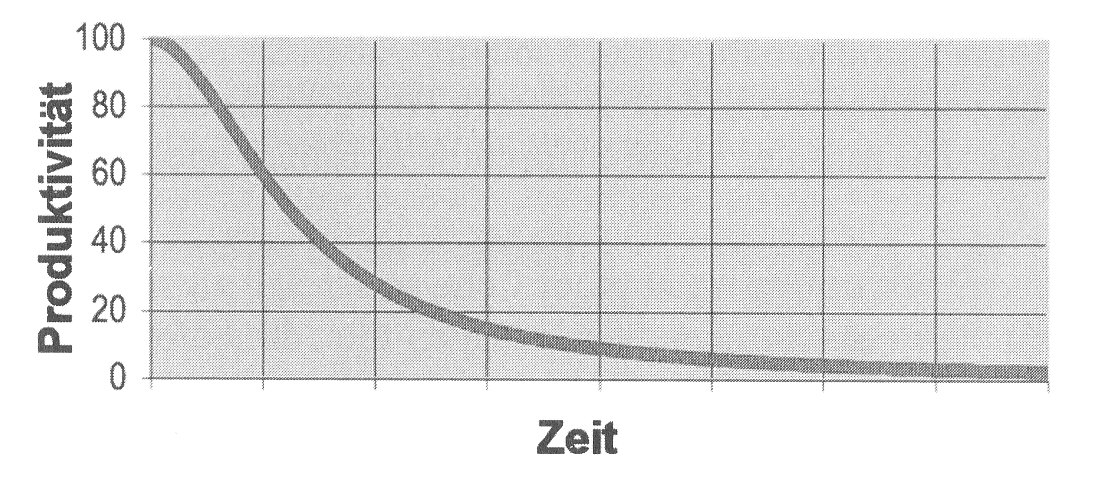
\includegraphics[width=\textwidth]{poduktivitaet.jpg}
	\caption{Produktivität über Zeit aus \cite[S. 29]{Martin}}
	\label{grundlagen:produktivitaet}
\end{figure}

Ein Entwickler der an einem solchen Quelltext arbeitet ist leicht versucht selbst schlechten Quelltext zu schreiben, da dies vermeintlich schneller geht und der Quelltext ohnehin schon nur schwer zu lesen ist. Daraus resultiert, dass der Quelltext immer unverständlicher wird und die Produktivität weiter sinkt.
Als möglicher Ausweg kommt eine Neuentwicklung der Software aus Sicht von \cite[S. 29f.]{Martin}, nicht in Frage.
Er begründet dies damit, dass neue Software neben der Weiterentwicklung der alten Erstellt werden muss und trotzdem auf denselben Funktionsumfang der alten Lösung kommen. Dies ist bei großen Softwareprojekten meistens nicht möglich, da bereit sehr viel Entwicklungszeit in das alte System geflossen ist und es zu teuer ist einen sehr großen Quelltext neu zu entwickeln. Als mögliche Lösung führt er an das jeder Entwickler versuchen sollten den Quelltext an den er gearbeitet hat sauberer als vorher zu hinterlassen. Er bezeichnet dies als Pfadfinderregel.

\subsection{Guter Quelltext}

Guten Quelltext zu schreiben ist etwas womit sich schon viele Entwickler beschäftigt haben\cite{Martin, Green, Spinellis, reed}.
\cite[S. 32f.]{Martin} hat sich mit den Aussagen von verschiedenen erfahrenen Entwicklern zu sauberem Quelltext auseinandergesetzt.
Er kommt zu folgenden Punkten für guten Quelltext:

\begin{itemize}
\item Testbar
\item Geradlinig, man erkennt den Zweck
\item Verständlich, einfach zu durchschauen, erwartungskonform
\item Keine versteckten Absichten
\item Gute Namen
\item Minimale Abhängigkeiten
\item Keine Redundanzen
\item Keine Fehler/Exceptions verstecken
\end{itemize}

Diese Punkte ähneln sehr stark den Design Ideen der Programmiersprache Python\cite{Peters}.
Wie anhand der Punkte zu erkennen ist, findet sich guter Quelltext auf verschiedenen Ebenen wieder. Auf unterster Ebene im Quelltext bis hin zur gesamten Architektur der Software. Häufig gehört allerdings ein hohes Maß an Erfahrung dazu einen guten Quelltext zu schreiben.


\subsection{Art and Science}

In vielen Artikeln zu dem Thema finden man die Wörter \enquote{Art} und \enquote{Science}. So z.B.
\enquote{Coding Guidlines: Finding the Art in Science} von \cite{Green} oder \enquote{Science and Art} von \cite[S. 669]{Knuth}.
Damit spielt man darauf an das manche Quelltexte sich so schön lesen und verstehen lassen, das es einer hohen Kunstfertigkeit bedarf sie zu schreiben. \cite[S. 669]{Knuth} zeigt, dass nicht nur die Informatik \enquote{Art} und \enquote{Science} in dieser weiße benutzt wird. Er fand es auch in einem Buch über die Grundlagen der Photographie und in der Einleitung eines Wörterbuches\cite[S. 669]{Knuth}.
Er zeigt zudem einen Wandel in der Verwendung des Wortes \enquote{Art}.
Früher war es üblich von einem gut ausgeführten Handwerk als Kunst zu reden.
Knuth zieht somit den Schluss, dass \enquote{Science} das Wissen ist und \enquote{Art} das angewandte wissen.
In unserem Fall ist das Programmieren das Handwerk und guter Quelltext die Kunst.
Weiterhin hat jeder Programmierer seinen eigenen Stil einen Quelltext zu schreiben.
Selbst Coding Conventions lassen dem Entwickler genug Freiraum für einen eigenen Schreibstil, da es nicht möglich ist alles mit ihnen zu definieren.





\section{Coding Guidelines: Finding the Art in Science}
Das erste Paper, dass in dieser Arbeit behandelt wird, trägt den Titel \enquote{ Coding Guidelines: Finding the Art in Science, What separates good code from great code?} von Robert Green und Henry Ledgard\cite{Green}. Die Autoren versuchen eigene Regeln, für das entwickeln von Quelltext aufzustellen. Das Ziel ist es den Programmierer in die Lage zu versetzen, einen Quelltext zu schreiben der schnell und einfach von anderen Programmierern gelesen, verstanden und erweitert werden kann. Das schließt mit ein, dass sich der Entwickler, ohne Kenntnis des Systems, schnell im gesamten Quelltext zurechtfinden kann. Dies ist vor allem in großen, langlebigen Softwareprojekten von Nöten, da hier eine gewisse Fluktuation bei den Entwicklern nicht auszuschließen ist\cite[S. 12]{Green}.

Beim erstellen der Regeln wird nicht auf bestimmte Entwicklungsumgebungen oder andere Tools Rücksicht genommen. Die Regeln sollen mit allen Editoren angewandt werden können.
\subsection{Monospace and the ASCII}
Als erstes wird bezug auf den Artikel von Kamp\cite{Kamp} genommen. Dieser stellte fest wie wenig sich das Aussehen von Quelltexten im Laufe der Zeit geändert hat und wie sehr es noch dem Schreiben mit einer Schreibmaschine ähnelt. Es wurden zwar viele nützliche Programme entwickelt die beim erstellen von Quelltexten helfen können, trotzdem ist er immer noch in Textform. Noch dazu wird immer eine Monospace Schriftart zur Darstellung verwendet. Dazu kommt noch das es kein klassischer Fließtext ist. Der verwendete Wortschatz ist stark eingeschränkt und es werden häufig mathematische Darstellungsformen gewählt \cite[S. 2]{Green}. Darum wir im Paper\cite{Green} vorgeschlagen für Quelltext eine tabellenartige Formatierung zu wählen um die Lesbarkeit zu erhöhen. Ein Beispiel hierfür ist in Listing \ref{paper1:table} zu sehen. Die \enquote{\texttt{case}}, sowie die \enquote{\texttt{break}} Anweisungen befinden sich in einer Spalte und die Aufrufe für die einzelnen Verzweigungspfade befinden sich in einer Spalte.

\begin{listing}[H]
    \begin{minted}{c}
char c1;
c1 = getChoice();
switch(c1) {
    case 'q': case 'Q': quit();                 break;
    case 'e': case 'e': enterPerson(content);   break;
    case 'd': case 'd': delPerson(content);     break;
    case 's': case 's': sortByName();           break;
    case 'l': case 'l': showAll();              break;
    case 'f': case 'f': searchByName(content);  break;
    case default: System.out.println(
        "--Invalid Command!!\n");
}
    \end{minted}
    \caption{Beispiel für tabellarische Darstellung von Quelltext aus \cite[S. 2]{Green}}
    \label{paper1:table}
\end{listing}



\ref{grundlagen:namensgebung}

\subsection{Naming}
\label{paper1:naming}
Als nächstes wenden Sich Robert Green und Henry Ledgard der Benennung von Elementen zu\cite[S. 3f.]{Green}. Die Benennung aller Elemente ist ein wichtiges belang bei der Entwicklung. Eine Sinnvolle Benennung hilft dem Leser eines Quelltextes sich in diesem zu Orientieren. Sie stellen hierzu die folgenden Regeln auf\cite[S. 4]{Green}:
\begin{itemize}
    \item Variablen- und Klassennamen sollen Nomen bzw. Nominalphrasen sein
    \item Klassennamen sind zusammenfassende Nomen (\texttt{Book})
    \item Variablennamen sind exakte beschreibende Nomen (\texttt{BookingNumber})
    \item Prozeduren sollten Verben bzw. Verbphrasen sein (\texttt{CalculateCost})
    \item Wertliefernde Methoden sollen Nomen Phrasen sein (\texttt{GetName})
    \item Boolesche Werte sollen Adjektive sein
    \item Für zusammengesetzte Namen sollte man sich an die englische Sprache halten
    \item Namen sollten aussprechbar sein
\end{itemize}

Auf diese weiße soll dem Leser zu jeder zeit klar sein, ob eine Operation, eine Variable oder eine Klasse hinter einem Namen steht. Die Namen sollen in einfachem Englisch gehalten sein.
Weiterhin sprechen sie an, dass das finden eines geeigneten Namen sehr schwierig sein kann. Ziel bei der Namensgebung soll sein, dass man aus ihnen die Konzepte der Software ablesen kann.

\subsection{Länge von Namen}
Bei der Namensgebung kann es sehr schnell dazu kommen, dass die Variablennamen lang werden. Um Namen aber kurz und prägnant zu halten soll der Kontext mit einbezogen werden. In Listing \ref{paper1:contextbasednames} ist ein Beispiel mit zu langen Namen zu sehen. Da sie zur Klasse \texttt{Circle} gehören, ist der \texttt{Circle}-Präfix überflüssig. Die Variablen gehören klar zur \texttt{Circle}-Klasse.
\cite[S. 4f.]{Green}
\begin{listing}[H]
    \begin{minted}{java}
class Circle {
    public Point circleCenter;
    public Point circleRadius;
}
    \end{minted}
    \caption{Beispiel für die Verkürzung von Variablennamen anhand des Kontextes}
    \label{paper1:contextbasednames}
\end{listing}
Green und Ledgard vertreten auch die These, dass besonders häufig genutzte Variablenamen sehr kurz sein sollen \cite[S. 6]{Green}, da dies mehr Klarheit schafft. Am besten sollte der Variablennamen lediglich aus einem Buchstaben bestehen.

\subsection{Struktur durch Whitespaces}
Der Quelltext soll durch Einrückung, Zeilenumbrüche und Leerzeilen strukturiert werden. Wie bereits besprochen kann man die Struktur und den Ablauf eines Programmes durch Einrückung hervorheben. Leerzeilen sollen nach \cite[S. 6f.]{Green} für die folgenden Zwecke eingesetzt werden:
\begin{itemize}
\item Beim Wechsel von vorbereitendem Quelltext, wie Variablendeklarationen, zu ausführenden Befehlen.
\item Vor und nach Klassen, Methoden und Funktionen
\item Um verschiedene logisch zusammenhängende Quelltextteile von einander abzugrenzen.
\end{itemize}
Ein Beispiel ist in Listing \ref{paper1:linebreaks} zu sehen. Dies ist ein Ausschnitt aus einem Lösungsansatz für das \enquote{Dining Philosophers Problem}\cite{Chandy}. Es sind drei, durch Leerzeilen getrennte Blöcke zu sehen. Es ist erkennbar, dass sich der erste Block Variablen vorbereitet, der Zweite die eigentlichen Ablauf durchführt und der Dritte die Rückgabe darstellt.
\begin{listing}[H]
\begin{minted}{c}
void* philo(void *args) {
    int *num = (int*) args;

    printf("%d hello\n", *num);
    while (1) {
        think(*num);
        eat(*num);
    }

    return NULL;
}
\end{minted}
\label{paper1:linebreaks}
\caption{Beispiel für den Einsatz von Leerzeilen zur Hervorhebung der Struktur}
\end{listing}

Leerzeilen können den Zusammenhang zwischen einzelnen Zeilen darstellen. Auf Ebene der Zeilen kann ein Leerzeichen verwendet werden um, dass lesen zu erleichtern und die Struktur darzustellen.
Nach Green und Ledgrad\cite[S. 7]{Green} sollen Leerzeichen nach jedem Komma stehen, sowie vor und nach nicht unären Operatoren. Der Memberoperator \enquote{\texttt{.}} bildet die Ausnahme. Er wird ohne separierende Leerzeichen verwendet. Zwischen Variablen und unärem Operator darf kein Leerzeichen sein. Ein Beispiel dieser Regeln ist in Listing \ref{paper1:spaces} 

\begin{listing}[H]
    \begin{minted}{java}
int i = 1;
int j = input.get();
i++; --j;
return i * j;
    \end{minted}
    \label{paper1:spaces}
    \caption{Beispiel Leerzeichen zur Trennung von Operationen}
\end{listing}

Zuletzt wird in \cite{Green} noch eingeräumt, dass es Sinn machen kann, wie in Listing \ref{paper1:spaces}, Zwei Befehle in eine Zeile zu schreiben.

\subsection{Struktur durch Einrückung}
Einrückung ist kann ein gutes Hilfsmittel sein um dem Leser beim verstehen von Quelltexten zu helfen. Nach \cite[S. 8]{Green} sollte bei einfachen Bedingungen die Klammerung weggelassen werden. Siehe dazu Listing \ref{paper1:withoutbraces}. Durch die Einrückung soll die Struktur deutlich werden, welcher Befehl gehört zu welcher Methode, welche Methode zu welcher Klasse, etc.

\begin{listing}[H]
    \begin{minted}{c}
if (result >= 90)
    cout << "Grade of A!";
else if (result >= 80)
    cout << "Grade of B";
else if (result >= 70)
    cout << "Sorry, grade of C";
else
    cout << "Not very good";
    \end{minted}
    \label{paper1:withoutbraces}
    \caption{Beispiel für sich ausschließende Verzweigung ohne Blockklammern aus \cite[S. 8]{Green}.}
\end{listing}

Wenn man bei langen Zeilen gezwungen ist, im Befehl einen Zeilenumbruch einzufügen, wird in \cite[S. 3]{Green} vorgeschlagen, dass die zweite Zeile entweder um eine Ebene eingerückt oder ausgerückt wird.

\subsection{Kommentare}
Green und Ledgard schreiben, dass Kommentare mit Bedacht eingesetzt werden sollen. Das Hauptaugenmerk soll auf dem Quelltext liegen, nicht auf den Kommentaren. Der Quelltext soll so geschrieben sein, dass seine Intention klar erkennbar ist. Bei einem solchen Quelltext ist es nicht nötig viele Kommentare zu verwenden. Kommentare sollen als zusätzliches Medium für die Kommunikation zwischen Autor und Leser des Quelltextes dienen und nur dann verwendet werden wenn es nicht möglich ist den Quelltext so klar zu gestallten, dass klar zu erkennen ist was er bezweckt. \cite[S. 9]{Green}


\subsection{Bewertung}

Das man eine Monospace Schriftart zum Schreiben eines Quelltextes verwendet ist keine neue Erkenntnis. Nur so lässt sich die Struktur des Quelltextes durch Einrückung darstellen. Auch tabellenartige Strukturen sind möglich. Eine Tabellenstruktur birgt aber verschiedene Nachteile. Wenn man dies auf eine \enquote{\texttt{Switch-Case}} Anweisung, wie in Listing \ref{paper1:table} anwendet und bei einer späteren Änderung des Quelltextes mehr als ein Befehl pro Zeile ausgeführt werden soll wird diese Struktur schnell sehr breit. Hinzu kommt bei allen Tabellenstrukturen, dass  Veränderungen häufig sehr schreibintensiv sind. Stelle man sich eine \enquote{\texttt{Switch-Case}} Anweisung vor, die viele verschiedene Fälle abdeckt. Fügen wir einen neuen hinzu, deren Methodenaufruf länger ist als die bereits vorhandenen Aufrufe, muss man die anderen Zeilen der Tabelle anpassen.

Die Richtlinien für Variablennamen funktionieren gut. Sie erfüllen klar ihren Zweck. Lediglich eine Erwähnung wie zusammengesetzte Variablennamen zu schreiben sind fehlt. In den Beispielen wurde immer eine \enquote{CamelCase} Variante gewählt. Der Variablenname \enquote{GetName} ließe sich auch als \enquote{Get\_Name} schreiben und hat eine äquivalente Bedeutung. Wenn nun verschiedene Entwickler am Quelltext arbeiten und der eine mit unterstrichen, der andere aber mit der \enquote{CamelCase} schreibweiße arbeitet wird der Quelltext schnell inkonsistent und wirkt nicht mehr einheitlich. Damit wäre das Ziel solcher vorgaben zunichte gemacht. Die Art der Schreibweiße sollte festgelegt sein, damit diese im gesamten Quelltext einheitlich ist.

Bei der Länge von Variablennamen wurde gesagt, dass diese so kurz wie möglich, bei häufig verwendeten Objekten bzw. Funktionen sogar lediglich ein Zeichen. Gute Variablennamen zu finden ist eine Kunst für sich. Ein Variablenname sollte klar wiederspiegeln was es für eine Variable ist. Für globale, häufig verwendete Elemente gilt dies besonders, aber ein einzelnes Zeichen ist nicht aussagekräftig genug. Wenn man eine Klasse erstellt die einen Vektor beschreibt sollte diese nicht \texttt{V} heißen sondern \texttt{Vector}. Namen die lediglich aus einem Zeichen bestehen sollten nur für Elemente verwendet werden, die lediglich in einem kurzen Ausschnitt des Quelltextes verwendet werden. Üblicherweise gehören hierzu Zählvariablen in Iterationen.

Wie in \cite[S. 3, 6-8]{Green} gut beschrieben ist sind Zeilenumbrüche und Leerzeichen bzw. Tabs ein wichtiges Mittel um den Quelltext lesbar zu gestallten. Verzweigungen und Strukturen lassen sich durch Einrückungen verdeutlichen und logisch zusammenhängende Blöcke unterteilen. Lediglich das weglassen von Blockklammern für Anweisungen innerhalb von \enquote{\texttt{if}}-Blöcken kann sich negativ auswirken. Wenn bei Änderungen am Quelltext aus der einen Anweisung mehrere werden müssen die Blockklammern ergänzt werden, ist dabei zu verschmerzen. Es können sich so aber schnell Fehler einschleichen, die schwer zu finden sind. Wenn man beim Schreiben einer solchen  Anweisung versehentlich hinter dem \enquote{\texttt{if}} ein Semikolon einfügt, wird der Quelltext weiterhin Kompilieren und sich ausführen lassen, die Einrückung suggeriert eine Verschachtelung, die aber nicht stattfindet, weil der \enquote{\texttt{if}} Block leer ist. Beispielhaft ist dies in Listing \ref{paper1:semicolonif} zu sehen. Die Operation \enquote{\texttt{buy()}} wird immer aufgerufen.

\begin{listing}[H]
    \begin{minted}{c}
if (action == "buy");
    buy();
    \end{minted}
    \label{paper1:semicolonif}
    \caption{Beispiel für eine fehlerhafte Verzweigung, ohne Blockklammern. \cite[S. 8]{Green}.}
\end{listing}

Bei Kommentaren im Quelltext beschreiben Green  und Ledgard richtig, dass Kommentare lediglich sparsam und mit Bedacht eingesetzt werden sollen\cite[S. 9]{Green}. Guter Quelltext sollte genau dies erfüllen. Er sollte gelesen werden können und ohne Kommentare verstanden werden. Dies gestaltet sich manchmal jedoch als schwierig. An solchen Stellen ist ein Kommentar ein legitimes Mittel um dem Leser eine Hilfe zu sein.



\section{Reading, Writing, and Code}
Das zweite Paper, welches in dieser Arbeit behandelt wird ist \enquote{Reading, Writing, and Code} von Diomidis Spinellis\cite{Spinellis}. In diesem Abschnitt werden die wesentlichen Teile der Arbeit zusammengefasst. Das Paper beschreibt die Schwierigkeiten, Quelltext zu schreiben, der von einfach zu lesen und verstehen ist. 

Spinellis geht zunächst von der Annahme aus, dass Quelltext wesentlich einfacher zu schreiben, als zu verstehen ist. Dies begründet er damit, dass es zur Lösung eins Problems viele verschiedene Lösungswege gibt. Der Autor ist sich beim Schreiben immer bewusst, welchen Weg er geht, während der Leser sich den Weg erst erschließen muss \cite[S. 85]{Spinellis}. Guter Quelltext zeichnet sich an dieser Stelle dadurch aus, dass der Leser den Gedanken des Autors gut nachvollziehen kann. Das Schreiben von gutem Quelltext nimmt aber meist mehr Zeit in Anspruch. Ferner zieht er den Schluss, dass sich guter Quelltext erst in der Zukunft, sprich bei der Wartung und Erweiterung des Quelltextes auszahlt\cite[S. 86]{Spinellis}. Hier bemängelt er auch, dass in der Lehre zu wenig auf das Schreiben von Programmen in einem realen Umfeld eingegangen wird. Es ist meist so, dass der Quelltext von einer Person, in einer Programmiersprache, für genau eine Zielplattform entwickelt wird. In einer realen Umgebung entwickelt aber mehrere Entwickler an einem Quelltext, der in verschiedenen Programmiersprachen entwickelt und auf verschiedenen Plattformen lauffähig sein muss. \cite[S. 86]{Spinellis}

Nach Spinellis gehören zu den am schwersten zu verstehenden Quelltexten zum einen Systemnahe Programme, wie Datenbank Systeme, Grafikengines, Betriebssystem Kernel, etc., und zum anderen Objekt-Orientierte-Programme, die eine unangemessene abstraktionstiefe besitzen. \cite[S. 86]{Spinellis}

Seine Erkenntnis ist es, dass es keinen einfachen Weg gibt, gut verständlichen Quelltext zu schreiben. Um einen solchen Quelltext zu schreiben benötig der Autor vor allem Erfahrung. Er muss wissen wie man einen Quelltext schreibt, auch mithilfe von Coding Conventions, und wann man die Coding Conventions brechen soll. \cite[S. 86]{Spinellis}

\subsection{Programmiersprachen und sauberer Quelltext}
Für Spinellis kann die Grammatik einer Programmiersprache dazu beitragen gut lesbaren Quelltext zu schreiben. Als Beispiele für diese Kategorie führt er C++, Java, Ada, und Perl an. Mit Fortran 77 lässt sich genauso guter Quelltext schreiben, es ist aber im Gegensatz zu den vorher aufgeführten Programmiersprachen aufwändiger. \cite[S. 87]{Spinellis}

Dazu kommt noch das einige Sprachen, wie C++, dem Entwickler Sprachfeatures zur Verfügung stellen die den Quelltext schnell unleserlich werden lassen können, \enquote{[...]there are languages that discourage you from writing bad code through the lack of \enquote{dangerous} features, and there are languages that give you more than enough rope to hang yourself and all your code’s future maintainers.}\cite[S. 87]{Spinellis}

Zu diesen Features zählt er u.a.:
\begin{enumerate}
\item die GoTo-Anweisung
\item Operatorüberladung
\item Pointer
\item Dynamische Speicherverwaltung 
\item C/C++ Präprozessor Makros
\end{enumerate}

Diese können den Leser mit Leichtigkeit in die Irre führen.

\subsection{Kommentare}
Kommentare sind für Spinellis ein wichtiges Werkzeug, um die Lesbarkeit eines Quelltextes zu erhöhen. Damit ein Kommentar jedoch wertvoll für den Leser wird, muss dieser klar formuliert sein. Sie können dem Leser so eine Hilfe beim verstehen des Zusammenhanges sein. Einfach die Bedeutung der nächsten Anweisung wiedergeben steigert nicht die Lesbarkeit. Zum anderen lassen sich auf diese Weiße automatisch technische Dokumentationen generieren, als Beispiel nennte er JavaDoc\footnote{s.a. http://www.oracle.com/technetwork/java/javase/documentation/index-jsp-135444.html}. Damit die Kommentare jedoch gut genug sind muss das erstellen dieser direkt beim Schreiben des Quelltextes geschehen. Zu einem späteren Zeitpunkt erstellte Kommentare sind häufig qualitativ weniger Wert. \cite[S. 88]{Spinellis}

\subsection{Vorschläge zum Schreiben von besserem Quelltext}
Um nun als Autor einen bessere Quelltexte zu schreiben, gibt Spinellis den Rat keine IDE zu verwenden, sondern einen Texteditor, wie VIM oder EMACS. Er begründet dies damit, dass ein Entwickler, der eine IDE verwendet, nur aus der Sichtweiße seiner IDE schreibt. Einem Leser mit einer anderen IDE oder einem Texteditor, kann es so erschwert werden den Quelltext zu lesen. Zudem sollte beim Einsatz einer IDE auch sichergestellt werden, dass der Quelltext nicht in einem Binärformat abgelegt wird. Nur dann kann dieser in einem Texteditor sinnvoll angezeigt werden. Als Nebeneffekt lässt sich ein Quelltext in Textform besser in einem Versionsverwaltungssystem ablegen. \cite[S. 88]{Spinellis}




\section{Eigener Ansatz}

In diesem Teil der Arbeit wird eine Coding Convention erstellt. Sie soll dafür sorgen, dass ein Quelltext, der von mehreren Entwicklern geschrieben wird, eine Einheitliche Form annimmt. Zudem soll durch den Einsatz der Coding Convention die Lesbarkeit und Verständlichkeit des Quelltextes gefördert werden. Als Zielprogrammiersprache wird Java verwendet. In den hier erstellten Code Conventions wird kein Wert darauf gelegt, die einzig richtige Vorlage für guten Quelltext zu sein. 


\subsection{Formatierung}
Zunächst einige allgemeine Festlegungen zur Formatierung des Quelltextes. Diese dienen dazu, ein einheitliches Textbild zu erhalten.

Der Zeichensatz der bei der Entwicklung verwendet werden muss ist UTF-8. Dieses wird von der Programmiersprache selbst vorgegeben. Durch die Verwendung, des UTF-8 Zeichensatzes, können die meisten länderspezifischen Umlaute und Sonderzeichen abgebildet werden. Des weiteren können so Umlautfehler vermieden werden.

Für die Einrückung werden vier Leerzeichen verwendet. Der Einsatz von Tabulatoren hätte den Vorteil, dass jeder Entwickler die Tiefe der Einrückung nach seinen Wünschen einstellen kann. Auf den Einsatz von Tabulatoren ist aber verzichtet worden, weil diese zu überlangen Zeilen führen können. Wenn ein Entwickler einen Quelltext schreibt und bei ihm ein Tabulator die Länge von zwei Leerzeichen hat, ist es für ihn möglich sehr viel längere Zeilen zu schreiben als ein Entwickler dessen Tabulatoren acht Leerzeichen lang sind ohne gegen die nächste Regel im bezug auf Zeilenlänge zu verstoßen.

Eine Zeile sollte nicht breiter als 120 Zeichen werden. Sollte eine Zeile länger werden kann diese an geeigneter Stelle umgebrochen werden. Die Fortsetzung wird doppelt, sprich acht Leerzeichen tief, eingerückt.

\subsubsection{Blöcke}
Der Inhalt von Blockklammern wird immer eingerückt. Die öffnende Blockklammer wird immer in derselben Zeile verwendet wie die dazugehörige Anweisung. Die schließende steht für sich alleine. Optionale Blockklammern bei Bedingungen und Schleifen sind immer zu setzen. Wenn es Sinnvoll ist, können Blockklammern zur Verdeutlichung des Quelltextes eingesetzt werden. In Listing \ref{own:blockopengl} ist ein Beispiel dazu zu sehen.

\begin{listing}[H]
    \begin{minted}{java}
gl.PushMatrix();
{
    gl.glTranslatef(width/2, height/2, 0); 
    gl.glRotatef(a, 0, 0, 0); 

    gl.glBegin(GL.GL_TRIANGLES); 
    gl.glColor4f(0.7, 0.1, 0.7, 0.8); 
    gl.glVertex3f(0, 0, 0); 
    gl.glVertex3f(0, 50, 0); 
    gl.glVertex3f(25, 0, 25); 
    gl.glEnd(); 
}
gl.PopMatrix();
    \end{minted}
    \caption{Einsatz von Blockklammern zur Verdeutlichung der Struktur am Beispiel von OpenGL}
    \label{own:blockopengl}
\end{listing}


Die Transformationsoperationen nach dem \enquote{\texttt{gl.PushMatrix}} Aufruf gelten lediglich bis zum entsprechenden nächsten \enquote{\texttt{gl.PopMatrix}} Aufruf. Da die angewandten Rotationen und Translationen lediglich zwischen den aufrufen von Bedeutung sind kann es zur Lesbarkeit beitragen diese in einen extra Block zu schreiben.

\subsubsection{Zeilenumbrüche und Leerzeilen}
Als Zeilenumbruch wird der UNIX Zeilenumbruch verwendet. Dies bedeutet lediglich ein Zeilenvorschub(\textbackslash n), ohne Wagenrücklauf(\textbackslash r).

Dieser ist nach jeder öffnenden Blockklammer \enquote{\{} und jedem Semikolon zwingend. Durch diese Vorgabe wird sichergestellt, dass jede Anweisung in einer eigenen Zeile steht. Dies gilt genauso für Annotationen. Nach jeder Annotation muss ein Zeilenumbruch eingefügt werden. In \texttt{\enquote{ENUM}s} muss nach jedem Kommata ein Zeilenumbruch sein.

Leerzeilen sollen dazu verwendet werden eine sichtbare Trennung zwischen logischen Blöcken zu erzeugen. Die Trennung sollte jedoch maximal aus einer Leerzeile bestehen. Daraus ergeben sich u.a. Leerzeilen an folgenden Positionen:

\begin{itemize}
\item Nach der \texttt{package} Deklaration
\item Ggf. zwischen Importanweisungen von verschiedenen Quellen
\item Nach den Importen
\item Ggf. zwischen der Deklaration von Klassenvariablen
\item Zwischen der Deklaration von Klassenvariablen und Methoden
\item Zwischen den Methoden, inneren Klassen und inneren \enquote{\texttt{ENUM}s}
\end{itemize}

Diese sollen die Lesbarkeit des Quelltextes erhöhen. Der Quelltext wirkt dadurch weniger komprimiert. Zudem sollen die Leerzeilen logische zusammenhänge hervorheben.

\subsubsection{Leerzeichen}

Um eine bessere Lesbarkeit einzelner Zeilen zu erlangen werden an bestimmten Stellen Leerzeichen eingefügt. Dieses geschieht analog zu den Vorschlägen von Green und Ledgard\cite[S. 7]{Green}. Demnach wird nach jedem Komma ein Leerzeichen eingefügt. Zudem vor und nach nicht unären Operatoren. Der Memberoperator \enquote{.} bildet ist hiervon ausgenommen. Beispiele sind in Listing \ref{paper1:spaces}, auf Seite \pageref{paper1:spaces} zu sehen.

\subsection{Dateiaufbau}
Der Name, Speicherort und Teile der Struktur sind bereits durch die Spezifikation der Java Programmiersprache vorgegeben. Der Aufbau innerhalb der Datei ist wie in Listing \ref{own:struct}  aufgebaut: Jede Datei beginnt mit der \texttt{package} Deklaration. Danach kommen die \texttt{Import} Anweisungen. Nun beginnt der Hauptteil der Datei, die Klasse, das Interface oder ein \texttt{ENUM}. Nach dieser darf es keine weiteren Elemente mehr geben. Auch wenn es die Java Spezifikation zuließe. Weitere Konstrukte müssen in eine separate Datei gelegt werden.

Die Reihenfolgen in einem Interface oder einem \texttt{Enum} sind trivial, da sie lediglich eine Art von Inhalt enthalten können. In Klassen kommen immer zuerst die Deklaration der Klassenvariablen, erst danach die Methoden und am Ende innere Klassen, Interfaces oder \texttt{Enums}.

Bei den Klassenvariablen kommen zuerst die Konstanten, gefolgt von den statischen Variablen und dann erst die Objektvariablen. Zwischen diesen Einheiten müssen Leerzeilen gesetzt sein.

Bei den Methoden kommen zuerst die Konstruktormethoden, gefolgt von statischen Methoden und am Ende die Objektmethoden. Die Reihenfolge der Methoden sollte so sein, dass im oberen Teil die Abstraktere und zum Ende hin immer speziellere Methoden stehen.

\begin{listing}[H]
    \begin{minted}{java}
package my.package;

import java.packet.Klasse;

public class HelloWorldPrinter {
    
    private static final String HELLO_TEXT = "hello";

    private static String lastMessage = null;

    private String name;

    public HelloWorldPrinter(String name) {
        this.name = name;
    }

    public static void sayHello(String name) {
        HelloWorldPrinter printer = new HelloWorldPrinter(name);
        printer.sayHello();
    }

    public void sayHello() {
        System.out.Println(HELLO_TEXT + " " + name);
    }

}
    \end{minted}
    \caption{Beispiel für die Struktur einer Quelltextdatei}
    \label{own:struct}
\end{listing}

\subsection{Namensgebung}
Die Namen für Objekte unterstehen denselben Regeln wie sie auch Green und Ledgard aufgestellt haben. Sie sind in Abschnitt \ref{paper1:naming} auf Seite \pageref{paper1:naming} beschrieben. Mit Ausnahme der Regel, dass globale, häufig verwendete Objekte Namen haben dürfen die lediglich aus einem Zeichen bestehen. Jedes Element soll einen Namen haben, der die Aufgabe des Elementes möglichst genau beschreibt. Damit sind in zusammengesetzten Namen, Begriffe wie Info, Data, Object, etc. zu vermeiden. Diese bieten zum einen keine weitere Information,  was die Bedeutung der Variable angeht und kann die Verständlichkeit negativ beeinflussen. In Listing \ref{own:namingmeta} sind zwei Variablendeklarationen zu sehen, anhand der Namen kann nicht unterschieden werden was der Unterschied zwischen diesen ist. Weiterhin soll bei zusammengesetzten Namen soll die \enquote{Camel Case} Schreibweise verwendet werden.

\begin{listing}[H]
    \begin{minted}{java}
Map person = getPerson();
Map personData = getPersonData();
    \end{minted}
    \caption{Beispiel für schlechte Variablennamen.}
    \label{own:namingmeta}
\end{listing}


Ein weiterer wichtiger Punkt ist, dass alle Namen aussprechbar sein müssen. Das hat den Effekt, dass sich diese besser merken lassen und die mündliche Diskussion über den Quelltext zwischen den Entwicklern vereinfacht. Die Entwickler müssen sich keine umständlichen Hilfsbezeichner ausdenken.

Weiterhin sollen die Namen suchbar sein. Diese Eigenschaft ist nicht für alle Namen notwendig, sollte aber für wichtige Elemente mit bedacht werden. Ein Negativbeispiel ist die Programmiersprache \enquote{Go}\footnote{s.a. http://golang.org/}. Wenn man versucht Informationen über die Programmiersprache mithilfe des Schlüsselwortes \enquote{Go} zu finden, wird man viele falsche Ergebnisse erhalten.

Namen sollten immer an die Problemdomäne angelehnt sein. Die Begriffswelt sollte sich im Quelltext wiederspiegeln. Damit können Sprachbarrieren zwischen Fachpersonal aus der Problemdomäne und den Entwicklern verringert werden.

\subsection{Kommentare}
Kommentare sollen zusätzliche Informationen zum Quelltext anbieten. Sie sollten dabei aber nicht zu geschwätzig sein. Genauso sollen sie keine unnötigen Informationen, wie eine Liste der Änderungen o.ä. enthalten. Ebensoweit sollen sie den geschriebenen Quelltext einfach wiederholen. Dies wäre zudem eine unnötige Redundanz.

In den Kommentaren darf die Lizenz der Software hinterlegt werden. Dies trägt zwar weder zur Lesbarkeit noch zur Verständlichkeit des Quelltextes bei, ist aber mitunter notwendiger Bestandteil und muss damit aufgeführt werden.

Wenn Kommentare verwendet werden sollte in ihnen, z.B. der Grund für eine Architekturentscheidung Dokumentiert sein. Der Entwickler kann so die Absicht die er verfolgt deutlich machen. Es können auch Warnungen sein. Es gibt Fälle, in denen der Aufruf einer Methode ungewollte Nebenwirkungen hat. Vor solchen, sofern sie nicht offensichtlich sind, muss gewarnt werden. Sogenannte \enquote{TODOs} sind ebenfalls erlaubt. Der Entwickler kann so unfertige stellen Kennzeichnen und beschreiben was noch zu erledigen ist.

Zuletzt noch die \enquote{JavaDoc} Kommentare. Sie dürfen verwendet werden. Aber auch hier gilt, diese mit Bedacht zu verwenden. Wenn die Bedeutung einer Variable oder einer Methode bereits aus ihrem Namen bzw. aus ihrer Signatur hervorgeht, kann dieser weggelassen werden. Genauso bei internen Operationen. Öffentliche Schnittstellen sollten hingegen mit \enquote{JavaDoc} Kommentaren versehen werden. Diese werden in der Regel von Entwicklern verwendet dich keinen tieferen Einblick in den Quelltext haben.


\subsection{Klassen}
Eine Klasse soll genau einem Zweck dienen. Dieser soll möglichst klar erkennbar sein und sich im Namen der Klasse wiederspiegeln. Ggf. soll der Zweck der Klasse im JavaDoc erläutert werden. Dies soll unter dem Einsatz des Single-Responsibility-Prinzips geschehen. Das Single-Responsibility-Prinzip sagt aus, dass eine Klasse genau einen Zweck haben soll. Daraus ergibt sich, dass es nur genau einen Grund geben darf die Klasse zu ändern. \cite[S. 176f.]{Martin}

Ein Hinweis auf das verletzen des Single-Responsibility-Prinzips ist es, wenn eine Klasse sehr lang wird. Sollte eine Klasse lang werden, muss darüber nachgedacht werden, ob diese möglicherweise mehrere Einsatzzwecken hat und aufgeteilt werden soll. Bei kleinen Klassen, mit lediglich einem Zweck, lässt sich dieser schnell erschließen, da sie aufgrund des geringeren Umfanges übersichtlicher ist.

\subsection{Methoden}

Bei Methoden wird das gleiche Ziel, wie auch bei Klassen verfolgt, sie sollen kurz und übersichtlich sein. Lange Methoden lassen sich in mehrere Kleinere zerlegen.

\begin{listing}[H]
    \begin{minted}{java}
public Product getProductByName(String name) {
    name = name.replace(" ", "+");
    name = name.trim();
    name = name.toLowercase();
    
    for (Product product : products) {
        if (!product.isActive()) {
            continue;
        }
        if (!name.equals(product.getName())) {
            continue;
        }
        return product;
    }
    throw new NoResultException();
}
    \end{minted}
    \caption{Lange Methode, die zwei Aufgaben erfüllt.}
    \label{own:methodlong}
\end{listing}

Die Methode in Listing \ref{own:methodlong} sucht ein Produkt  anhand seines Namens. Dies geschieht in zwei Schritten. Zunächst wird der Parameter \texttt{name} auf die Suche vorbereitet, danach wird dieser in allen aktiven Produkten gesucht. Diese zwei Schritte können in zwei extra Methoden ausgegliedert werden. Ein mögliches Ergebnis ist in Listing \ref{own:methodshort} zu sehen. Die Methode ist stark verkürzt und man kann sehr schnell sehen, was die Methode wie erledigt.

\begin{listing}[H]
    \begin{minted}{java}
public Product getProductByName(String name) {
    name = prepareProductName(name);

    for (Product product : products) {
        if (isProductNameMatching(product, name)) {
            return product;
        }
    }
    throw new NoResultException();
}
    \end{minted}
    \caption{Gekürzte Version des Listings \ref{own:methodlong}}
    \label{own:methodshort}
\end{listing}

Ein weiterer wichtiger Aspekt an den Methoden ist die Parameteranzahl. Diese sollte möglichst gering sein und maximal 3 Parameter besitzen. Viele Parameter sind häufig ein Anzeichen dafür, dass eine Methode zu viele Aufgaben erledigt. Hier soll erwähnt sein, dass der Einsatz von Datenobjekten ausdrücklich erlaubt ist.

\enquote{Flag}-Parameter, die das Verhalten einer Methode beeinflussen sind nicht erlaubt. Sie schaden der Lesbarkeit des Quelltextes. In Listing \ref{own:flag} ist ein Methodenaufruf zu sehen. Dabei ist die Bedeutung des übergebenen Parameters nicht erkennbar. Besser ist es in einem solchen Fall zwei Methoden zu schreiben. Eine die das Verhalten mit gesetztem Flag, eine ohne abbildet. Der Name der Methode muss dieses Verhalten natürlich wiederspiegeln.

\begin{listing}[H]
    \begin{minted}{java}
item.publish(true);
    \end{minted}
    \caption{Beispiel für einen \enquote{Flag}-Parameter}
    \label{own:flag}
\end{listing}

Die verschachtelungstiefe kann ein weiterer Anhaltspunkt für zu komplexe, schwer zu lesende Methoden sein. Wenn eine Methode tief verschachtelt ist, zeugt dies von einer höheren Komplexität als flache Methoden, was sich u.a. in der zyklomatischen Komplexität wiederspiegelt\cite{McCabe}. Es gibt verschiedene Verfahren um die verschachtelungstiefe gering zu halten. Die offensichtlichste ist es, den Quelltext in verschiedene Methoden aufzuteilen. Eine andere Möglichkeit ist es in geeigneten Fällen, eine frühe Rückkehr aus der Methode zu verwenden. Listing \ref{own:lowindent} zeigt wie dies anhand von Validierungsoperationen. Sobald ein Fehler erkannt bemerkt wurde, wird die Methode sofort verlassen.

\begin{listing}[H]
    \begin{minted}{java}
void print(String text) {
    if (text == null) {
        return;
    }
    if (text.isEmpty()) {
        return;
    }
    System.out.Println(text);
}
    \end{minted}
    \caption{Beispiel für das frühzeitige verlassen einer Methode um eine niedrige Verschachtelungstiefe zu erhalten.}
    \label{own:lowindent}
\end{listing}

\subsection{Fehlerbehandlung}
Bei der Fehlerbehandlung sind Exceptions zu verwenden. Die Rückgabe von Fehlercodes oder \texttt{NULL} werten ist verboten. Fehlercodes und \texttt{NULL} Werte bieten keinen Vorteil gegenüber von Exceptions, welche genau für den Ausnahmefall entworfen sind. 

In Listing \ref{own:methodnull} ist der Aufruf ein Methodenaufruf zu sehen, der einen \texttt{NULL} wert zurückgibt, in Listing \ref{own:methodexception} anstelle von \texttt{NULL} eine Exception geworfen.

\begin{listing}[H]
    \begin{minted}{java}
List<Product> products = getProducts();
if (products == null) {
     // handle
}
    \end{minted}
    \caption{Methodenaufruf mit \texttt{NULL} Rückgabewert}
    \label{own:methodnull}
\end{listing}

\begin{listing}[H]
    \begin{minted}{java}
try {
    List<Product> products = getProducts();
} catch (EmptyResultException exception) {
    // handle
}
    \end{minted}
    \caption{Methodenaufruf mit Exception}
    \label{own:methodexception}
\end{listing}

Die Methodenaufrufe ähneln einander zwar, aber im Listing \ref{own:methodexception} wird dem Leser erst deutlich gemacht was passiert. Am Namen der Exception ist klar zu erkennen welche Ausnahme an dieser Stelle behandelt wird, nämlich das es keine Produkte gibt. In Listing \ref{own:methodnull} ist nicht zu erkennen was schief gelaufen ist, sprich weshalb die Methode kein Ergebnis liefert.

\subsection{Magic-Strings and Numbers}
Magic –Strings sind feste Zeichenketten bzw. Zeichen, welche fest in den Quelltext eingebaut sind. Solche Werte werden häufig für bestimmte Zustände verwendet. Listing \ref{own:magicstrings} zeigt einige Beispiele.

\begin{listing}[H]
    \begin{minted}{java}
search(searchString, 3);        
call("GET", document);
respones(404);
    \end{minted}
    \caption{Beispiel für Magic-Strings}
    \label{own:magicstrings}
\end{listing}


Die Bedeutung der festen Werte wird dem Leser nicht deutlich gemacht. Was bedeutet die \enquote{3} in der \texttt{search} Methode? Es ist nicht ersichtlich welchen Einfluss dieser Wert auf die Ausführung nimmt. Für solche Fälle müssen Konstanten mit entsprechenden Namen erzeugt werden. Dies bietet gleich zwei Vorteile. Erstens wird der konstante wert nur einmal im Quelltext verwendet, an der Stelle an der die Konstante deklariert wird, dadurch lassen sich spätere Änderungen leicht durchführen. Zweitens kann der Leser nun erkennen was an die Methoden übergeben wird und sich ihre Bedeutung erschließen. In Listing \ref{own:magicstringsconst} sind die werte durch Konstanten getauscht.

\begin{listing}[H]
    \begin{minted}{java}
search(searchString, SearchParameter.TO_LOWER_CASE);
call(Http.GET, document);
respones(HttpCodes.PAGE_NOT_FOUND);
    \end{minted}
    \caption{Magic-Strings durch konstanten ersetzen}
    \label{own:magicstringsconst}
\end{listing}





\section{Fazit}

Einen guten Quelltext zu schreiben ist eine Komplizierte Angelegenheit. Es reicht nicht aus, dass der Quelltext lediglich die gestellte Aufgabe löst. Er muss vielmehr durch einen klaren Schreibstil und eine klare Ausdrucksweise, dem Leser seine Intention in jedem Detail deutlich machen. Das gilt für sowohl für die kleinsten Implementierungsdetails, wie auch für das große Gesamtbild der Software.

Zu einem guten Quelltext gehört genauso eine angemessene Architektur, welche die abstrakte Arbeitsweiße der Software deutlich macht. Der große Unterschied zwischen Mensch und Maschine ist nun einmal, dass die Maschine lediglich den Quelltext abarbeiten muss, der Mensch ihn aber verstehen möchte.

Deshalb ist es so schwer eine gute Coding Convention zu erstellen. Es gibt keine universelle ausdrucksweiße, die jeder Mensch gleichermaßen schnell verstehen kann. Dazu kommt noch, dass beim Schreiben eines Quelltextes, der Autor, das Problem schon verstanden und einen Lösungsweg im Kopf hat. Wenn der Autor einen neuen Quelltext schreibt, muss er sich nicht mit dem Quelltext und damit den Lösungswegen von anderen Autoren herumschlagen. Er kann sich vielmehr ausschließlich auf die Problemlösung konzentrieren. In der Realität ist dies aber sehr selten der Fall. Meistens ist es so, dass an ein bereits vorhandener Quelltext weiterentwickelt bzw. gewartet wird. Dabei muss sich der Autor häufig mit dem Quelltext von anderen Autoren auseinander setzen. 

Damit ein Autor einen guten Quelltext schreiben kann, muss er selbst schon viele Quelltexte gelesen und geschrieben haben, damit er weiß, wie schwer es sein kann einen Quelltext zu verstehen.

Eine Coding Convention kann nicht alleine dafür sorgen, dass man einen guten Quelltext erhält. Sie kann lediglich als Richtlinie dienen um eine einheitliche Formatierung zu gewährleisten. Einen wirklich guten Quelltext zu schreiben gehört zu einer hohen Kunst in der Zunft der Softwareentwickler.




\appendix

\newpage

\nocite{*}
 
\printbibliography
\addcontentsline{toc}{section}{Literatur}

\newpage
 
\addcontentsline{toc}{section}{Abbildungsverzeichnis}
\listoffigures

\newpage
 
\addcontentsline{toc}{section}{Quellcodeverzeichnis}
\renewcommand\listoflistingscaption{Quellcodeverzeichnis}
\listoflistings

\end{document}
